\documentclass[a4paper]{article}
\linespread{1.6}
\usepackage{floatrow}
\floatsetup[table]{capposition=top}  
\newfloatcommand{capbtabbox}{table}[][\FBwidth] 
\usepackage{enumerate}
\usepackage{comment}
\usepackage{geometry}
\usepackage{setspace}
\usepackage{amsmath}
\usepackage{amssymb}
\usepackage{algorithm}
\usepackage{algorithmicx}
\usepackage{algpseudocode}
\usepackage[pdftex]{graphicx}
\usepackage{float}
\usepackage{subfigure}
\usepackage{listings}
\usepackage{algpseudocode}
\geometry{left=1.2cm,right=1.2cm,top=2.5cm,bottom=2.5cm}

%\floatname{algorithm}{Algorithm}
%\renewcommand{\algorithmicrequire}{\textbf{Input:}}
%\renewcommand{\algorithmicensure}{\textbf{Output:}}

\begin{document}
\begin{spacing}{2.0}
\begin{flushleft}\begin{huge}EEE6512 Image Processing and Computer Vision   Homework 4\end{huge}\end{flushleft}
\begin{flushright}\begin{Large} Hudanyun Sheng \end{Large}\end{flushright}

\section*{\huge\textbf{ Part \uppercase\expandafter{\romannumeral1} Textbook Questions}  }
	\normalsize
	\noindent
	
	10.1 Segmentation corresponds to which branch of machine learning?

	Segmentation corresponds to unsupervised machine learning.\\
	

	10.6 Compute the optimal threshold for the following grayscale image using (a) the Ridler- Calvard algorithm and (b) Otsu's method:
	$$\begin{bmatrix}
	6 & 5 & 8 & 7\\
	4 & 2 & 3 & 8\\
	1 & 8 & 6 & 1\\
	\end{bmatrix}$$ 
	
	The histogram of this grayscale image: $h = [0 \ \ 2 \ \ 1 \ \ 1 \ \ 1 \ \ 1 \ \ 2 \ \ 1 \  \ 3]$
	\begin{enumerate}
	\item[(a)] Ridler - Halvard algorithm: \\
	$\xi = 9$, $\tau = 4$, thus, $\mu_{\blacktriangleleft} = 0+2+1+1+1 = 5$, $\mu_{\vartriangleright} = 1+2+1+3 = 7$.\\
	Thus, update $\tau = (5+7)/2 = 6$. $\mu_{\blacktriangleleft} = 0+2+1+1+1+1 +2  = 8$, $\mu_{\vartriangleright} = 1+3 = 4$.\\
	Thus, update $\tau = (8+4)/2 = 6$. The $\tau$ remains unchanged, so the final threshold is found: $\tau = 6$.
	
	\item[(b)] Otsu's method: the goal for us is to maximize the between class variances:
	$$\sigma_b^{2}(\tau) = p_{\blacktriangleleft}(\tau)(\mu_{\blacktriangleleft}(\tau)-\mu)^2+p_{\vartriangleright}(\tau)(\mu_{\vartriangleright}(\tau)-\mu)^2$$
	where $\mu = \displaystyle\frac{1}{12}(0\times 0+1\times 2+2\times 1+3\times 1+4\times 1+5\times 1+6\times 2+7\times 1+8\times 3) = \displaystyle\frac{59}{12}\approx 4.92$.t \\
	$\sigma_b^{2}(0) = 0\times(0-4.92)^2+1\times(4.92-4.92)^2 = 0$, \\
	$\sigma_b^{2}(1) = (2/12)\times(2/2-4.92)^2+(10/12)\times((2+3+4+5+12+7+24)/10-4.92)^2 = 3.0681$,\\
	$\sigma_b^{2}(2) = (3/12)\times((2+2)/3-4.92)^2+(9/12)\times((3+4+5+12+7+24)/9-4.92)^2 = 4.2801$, \\
	$\sigma_b^{2}(3) = (4/12)\times((2+2+3)/4-4.92)^2+(8/12)\times((4+5+12+7+24)/8-4.92)^2 = 5.0139$, \\
	$\sigma_b^{2}(4) = (5/12)\times((2+2+3+4)/5-4.92)^2+(7/12)\times((5+12+7+24)/7-4.92)^2 = 5.2716$, \\
	$\sigma_b^{2}(5) = (6/12)\times((2+2+3+4+5)/6-4.92)^2+(6/12)\times((12+7+24)/6-4.92)^2 = 5.0625$, \\
	$\sigma_b^{2}(6) = (8/12)\times((2+2+3+4+5+12)/8-4.92)^2+(4/12)\times((7+24)/4-4.92)^2 = 4.0139$, \\
	$\sigma_b^{2}(7) = (9/12)\times((2+2+3+4+5+12+1)/9-4.92)^2+(3/12)\times((24)/3-4.92)^2 = 1.0890$, \\
	$\sigma_b^{2}(8) = 1\times((2+2+3+4+5+12+1+24)/12-4.92)^2+0\times(0-4.92)^2 = 0$, \\
	Based on the calculation above, the final threshold is found $\tau = 4$.
	\end{enumerate}
	
	10.7 On the same image of the previous problem, compute the threshold using the following adaptive thresholding algorithms with a 3$\times$3 sliding window: (a) Equation (10.19), (b) Niblack's method, and (c) Sauvola's method. For simplicity, show results only for the middle two pixels, use a box filter, and set t=0.8, k=0.2, and r=4.\\
	The $3\times 3$ window of the left and right middle pixels are: 
	
	$\begin{bmatrix}
	6 & 5 & 8\\
	4 & 2 & 3\\
	1 & 8 & 6
	\end{bmatrix}$, with $\mu_1 = 4.7778$ and $\sigma_1 = 2.4889$, \\
	and $\begin{bmatrix}
	5 & 8 & 6\\
	2 & 3 & 8\\
	8 & 6 &1
	\end{bmatrix}$, with $\mu_2 = 5.3333$ and $\sigma_2 = 2.7386$
	\begin{enumerate}
	\item[(a)]Equation (10.19): $\tau(x,y) = t \times \mu(x,y)$.\\
	$t = 0.8$, thus $\tau(1,1) = t\times \mu_1 = 0.8\times 4.7778 = 3.8222$ (left center pixel), $\tau(2,1) = t\times \mu_2 = 0.8\times 5.3333 = 4.2666$ (right center pixel).
	
	\item[(b)]Niblack's method: $\tau(x,y) = \mu(x,y) - k\sigma(x,y)$.\\
	$k = 0.2$, thus $\tau(1,1) = \mu(1,1) - k\times \sigma(1,1) = 4.7778 - 0.2\times 2.48889 = 4.2800$ (left center pixel), $\tau(2,1) = \mu(2,1) - k\times \sigma(2,1) = 5.3333 - 0.2\times 2.7386 = 4.7856$ (right center pixel).
	
	\item[(c)] Sauvola's method: $\tau(x,y) = \mu(x,y)[1-k(1-\displaystyle\frac{\sigma(x,y)}{r})]$, $k = 0.2$, $r = 4$.\\
	$\tau(1,1) = \mu(1,1)[1-0.2(1-\displaystyle\frac{\sigma(1,1)}{4})] = 4.7778[1-0.2(1-\displaystyle\frac{2.4889}{4})] = 4.4168$.\\
	$\tau(1,2) = \mu(1,2)[1-0.2(1-\displaystyle\frac{\sigma(1,2)}{4})] = 5.3333[1-0.2(1-\displaystyle\frac{2.7386}{4})] = 4.9969$.\\
	\end{enumerate}
	
	10.9 Perform hysteresis thresholding on the following image with a low threshold of 3 and a high threshold of 7 (that is, I(x,y) $>$ 3 and I(x,y)$>$ 7) to reveal an important concept in segmentation:
	\begin{figure}[htbp]
	 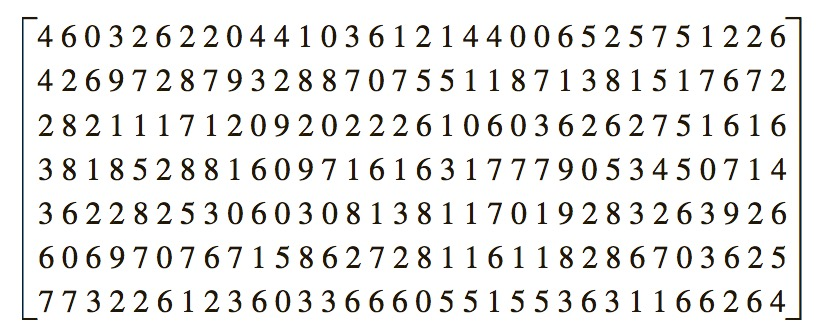
\includegraphics[width=4in]{p9.jpg}
	\end{figure}

	With the low threshold I(x,y) $>$ 3, the result is shown below (for convenience, use black to represent 1, white to represent 0):
	\begin{figure}[htbp]
	 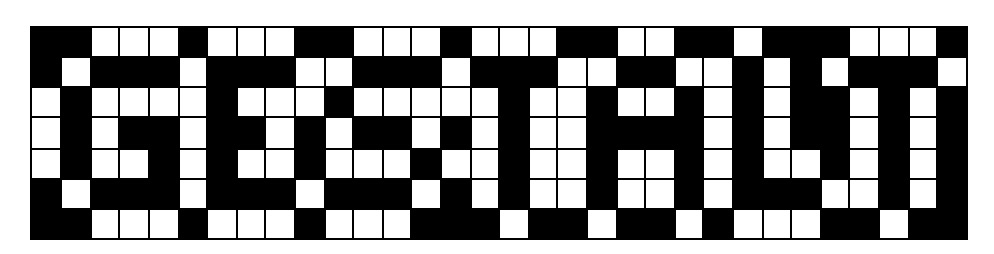
\includegraphics[width=4in]{low.jpg}
	\end{figure}
	
	With the high threshold I(x,y) $>$ 7, the result is shown below (for convenience, use black to represent 1, white to represent 0):
	\begin{figure}[htbp]
	 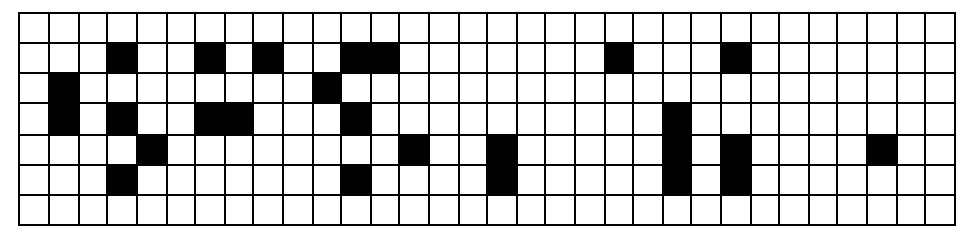
\includegraphics[width=4in]{high.jpg}
	\end{figure}
	
	And the final result with hysteresis thresholding is shown below:
	\begin{figure}[H]
	 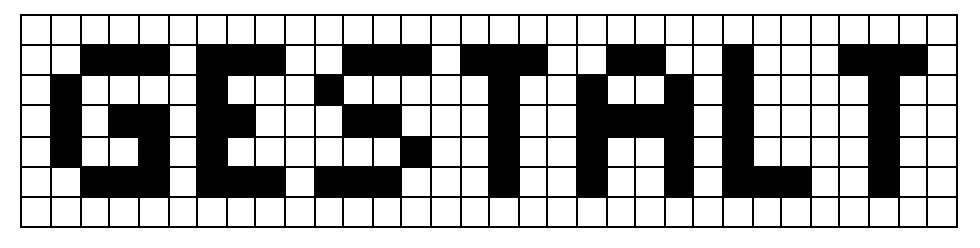
\includegraphics[width=4in]{result.jpg}
	\end{figure}
	It is ``GESTALT".
	
	10.10 Apply morphological reconstruction by dilation, Equation(10.22), to the image of the previous question and compare the results.
	
	The result image would be the same, since it is mentioned in the textbook that the hysteresis thresholding can be represented as morphological reconstruction $I' = T_{high}\textcircled{+}^*T_{low}B$. So the results would remain the same.\\

 	10.32 What is the difference between agglomerative clustering and divisive clustering?
For each of the following algorithms, specify whether it is an agglomerative or divisive approach: (a) region growing, (b) watershed, (c) mean shift segmentation, (d) Felzenszwalb- Huttenlocher, (e) normalized cuts, and (f ) minimum s-t cut.

	Agglomerative clustering begins with each pixel as a separate region and iteratively joins pixels until converge. Divisive clustering begins with the entire image as a single region and iteratively split the region until convergence.\\
	Agglomerative clustering: (a), (b), (c), (d).
	Divisive clustering: (e), (f).\\
	
	10.37 Draw the dendrogram corresponding to the graph in Figure 10.32, assuming single-link clustering.
	
	10.38 Explain the primary drawback of tobogganing.
	
	The drawback of tobogganing, as mentioned in the textbook is that discretization effects in a digital image make it impossible to determine the downward direction using only local information when there is a plateau.\\
	
	10.43 Describe the relationship between mean-shift filtering and mean-shift segmentation.
	
	Mean-shift filtering: a smoothing method, and it is actually an anisotropic method, transform an image into a cartoon-like output image.\\
	Mean-shift segmentation: a segmentation method which used mean-shift filtering to segment images.
	
	
\newpage	
\section*{\huge\textbf{ Part \uppercase\expandafter{\romannumeral1} MATLAB Programming}  }
	\normalsize			
	The MATLAB code of function ``regiongrow-seg" is attached as a commented M-file.
	
\end{spacing}
\end{document}